\section{有补格}
一般来说,偏序格\(L\)不一定存在最大元与最小元.
例如实数集\(\mathbb{R}\)关于小于等于关系\(\leq\)的偏序格\(\opair{R,\leq}\).

\begin{definition}
%@see: 《离散数学》(邓辉文) P159 定义5-24
设\(\opair{L,\leq}\)是偏序格.
若\(L\)存在最大元和最小元,
则称“\(\opair{L,\leq}\)是\DefineConcept{有界格}(bounded lattice)”.
\end{definition}

按偏序集中的约定:
有界格的最大元记为\(1\),最小元记为\(0\).

由定义可知,在有界格\(\opair{L,\leq}\)中,
对任意\(x \in L\),有\(0 \leq x \leq 1\).
进而有\begin{gather*}
	x + 1 = 1, \\
	x \cdot 1 = x, \\
	x + 0 = x, \\
	x \cdot 0 = 0.
\end{gather*}
于是,\(1\)是\(\opair{L,\cdot}\)的单位元,
\(0\)是\(\opair{L,+}\)的单位元.

\begin{example}
%@see: 《离散数学》(邓辉文) P159 例5-33
设\(X\)是非空集合.
证明:\(\opair{\Powerset X,\subseteq}\)是有界格.
%TODO proof
\end{example}

\begin{proposition}
%@see: 《离散数学》(邓辉文) P159
任意有限格是有界格.
%TODO proof
\end{proposition}

\begin{definition}
%@see: 《离散数学》(邓辉文) P159 定义5-25
设\(\opair{L,+,\cdot}\)是有界格,
\(a \in L\).
若存在\(b \in L\)使得\(a + b = 1\)且\(a \cdot b = 0\),
则称“\(b\)是\(a\)的\DefineConcept{补元}”.
\end{definition}

显然,在任意有界格中,若\(b\)是\(a\)的补元,则\(a\)是\(b\)的补元;
\(0\)与\(1\)互为补元;
但是,不是每个元素都有补元,同一个元素的补元未必唯一.

\begin{example}
%@see: 《离散数学》(邓辉文) P159 例5-34
讨论哈斯图 \labelcref{figure:格论.偏序集4} 所示的偏序格中每个元素的补元.
\begin{figure}[hbt]
%@see: 《离散数学》(邓辉文) P159 图5-6
	\centering
	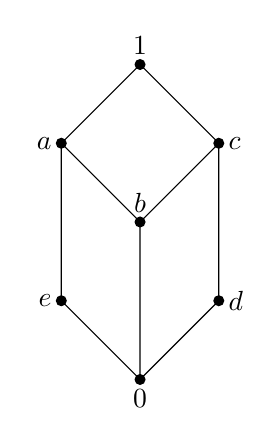
\begin{tikzpicture}
		\fill(0,0)circle(2pt)node[above]{$1$};
		\fill(1,-1)circle(2pt)node[right]{$c$};
		\fill(1,-3)circle(2pt)node[right]{$d$};
		\fill(0,-4)circle(2pt)node[below]{$0$};
		\fill(-1,-3)circle(2pt)node[left]{$e$};
		\fill(-1,-1)circle(2pt)node[left]{$a$};
		\fill(0,-2)circle(2pt)node[above]{$b$};
		\draw(0,0)--(1,-1)--(1,-3)--(0,-4)--(-1,-3)--(-1,-1)--(0,-2)
			(0,0)--(-1,-1) (0,-4)--(0,-2)--(1,-1);
	\end{tikzpicture}
	\caption{}
	\label{figure:格论.偏序集4}
\end{figure}
\begin{solution}
\(0\)与\(1\)互为补元.
\(a\)的补元是\(d\).
\(b\)的补元不存在.
\(c\)的补元是\(e\).
\(d\)的补元是\(a\)和\(e\).
\(e\)的补元是\(c\)和\(d\).
\end{solution}
\end{example}

\begin{example}
%@see: 《离散数学》(邓辉文) P159 例5-35
设\(X\)是非空集合.
证明:\(\opair{\Powerset X,\subseteq}\)是有补格.
%TODO proof
\end{example}

\begin{example}
%@see: 《离散数学》(邓辉文) P159
设\(F\)是全体合式公式,\(\implies\)是逻辑蕴含关系.
证明:\(\opair{F,\implies}\)是有补格.
%TODO proof
\end{example}
